% !TEX root = ../master.tex
\chapter{Fundamentals}
\label{chap:fund}

\section{\acl{BIA}}

Chen et.~al characterize \ac{BIA} as \blockcquote[p.~1166]{chen2012business}{the techniques, technologies, systems, practices, methodologies, and applications that analyze critical business data to help an enterprise better understand its business and market and make timely business decisions}. Its goals and methodology closely resembles that of the emerging field of \ac{BDA} \autocite[][p.~1166]{chen2012business}. 
According to Chen et.~al and their involvement in the \ac{BIA} space from the end of the last century to the 2010s three major evolutionary phases of the sector may be differentiated, with \ac{BDA} characterizing the evolution in the last stage \autocite[][p.~1168 \psqq]{chen2012business}. In order to provide an overview regarding the development of the context area, the different stages will be looked at and briefly characterized hereafter.

In the first evolutionary phase, identified as \textbf{\ac{BIA} 1.0}, the desire for the storage and analysis of business data emerged. Companies started to utilize already existing \acp{RDBMS} to store mostly structured data collected from various legacy systems such as mainframes. This phase includes the usage of statistical methods to generate and validate new hypotheses regarding stored information, widely known as \ac{DM}. In this regard the main emphasis of \ac{BIA} departments was to design, deploy and maintain data warehouses with optimized \ac{ETL} cycles in order to regularly feed new data into the system using batch processing. The stored information may then be analyzed using \ac{OLAP} systems and are usually visualized with dashboards and graphs to allow a better insight for the end-users.
Most of the currently deployed analytic platforms, including standard software by common software vendors such as Microsoft or Oracle, are based on the technologies developed in the \ac{BIA} 1.0 phase. Although these developments already started in the 1970s and accelerated in the 1980, there is still ongoing research and active feature implementation until today. \autocite[][p.~1166 \psq]{chen2012business}

As the Web 2.0 became popular in the early 2000s, an unknown variety of data sources emerged as well. The goal of the \textbf{\ac{BIA} 2.0} ignited by these events is to harvest the new opportunities for analytical processing created by this additional data. The collection of statistics on an individual customer basis allowed to generate a better understanding of customer's needs and thus offer tailored goods and services to a company's clients.
Moreover, the invention of social media platforms led to a massive influx of publicly available user-generated content. The analysis of such unstructured data posed the main challenge to traditional applications, focused on structured data with well-defined schemes. Although some techniques and opportunities addressed by \ac{BIA} 2.0 have been incorporated into commercial offerings, there still exists a large room for future growth. Especially the techniques of text mining, social network and spatial-temporal analysis are still under active academic investigation. \autocite[][p.~1167 \psq]{chen2012business}

Finally, the most interesting phase in the context of \ac{BDA} is that of \textbf{\ac{BIA} 3.0}. Sparked by an exponentially increasing volume of data due to mobile and \ac{IoT} devices, that \enquote{traditional} systems are not capable of dealing with, this term represents a new research area currently in development. The enormous desire of enterprises to gain meaningful insight from the \blockcquote[p.~1168]{chen2012business}{massive, location-aware, person-centered and context-relevant data} in a so-called Web 3.0 environment is leading both IT vendors and academia to develop tailor-fit solutions. However, as of today,  no comprehensive standard software is commercially available yet, and neither are academic courses that educate the workforce of tomorrow. \autocite[][p.~1168]{chen2012business}


\section{\acl{BDA}}
Rajasekar et. al. establishes a understanding on the definitions and tools of \ac{BDA}, enriched by offering a comparison with traditional \acp{DBMS} regarding size and type of the underlying input data \autocite[][p.~80]{rajasekar2015survey}. Accordingly, \ac{BDA} is concerned with the analysis of the \enquote{massive amount of un-, semi- and structured data too large to be handled by traditional DBMS}. The property of being too large is therefore strongly dependent on the precise \ac{DBMS} in use \autocite[][p.~80]{rajasekar2015survey}, and the threshold level might change in the future as technological advancements enable legacy software to process larger data quicker. However, additional processing power created by technological advancements is unlikely to keep up with the exponential growth of incoming data. \autocite[][p.~80\psq]{rajasekar2015survey}

\begin{table}[hbt]
	\begin{tabular}{l|ll}
	  \textbf{Characteristic} & \textbf{Traditional \acp{RDBMS}} & \textbf{\acf{BDA}} \\[0.5em]
	  \hline
	  Data Size & Gigabytes & Petabytes \\
	  Access Type & Interactive and Batch & Batch only \\
	  Update Frequency & Continuously Read and Write & Write once, Read continuously \\
	  Schema Type & Static & Dynamic \\
	  Data Integrity & High & Low \\
	  Scaling Behavior & Nonlinear & Linear \\
	\end{tabular}
	\caption{Comparison of typical \acl{RDBMS} and \acl{BDA} properties. Reprinted with adaptions from \autocite[][p.~80]{rajasekar2015survey}}
	\label{fig-dbms-vs-bda}
\end{table}


In order to compare the most important properties of traditional \acp{RDBMS} with those of
\ac{BDA} methods, i.e. \emph{MapReduce}, the authors propose a table similar to
\autoref{fig-dbms-vs-bda}. The table highlights the flexibility that is connected with \ac{BDA},
achieved by breaking up the structure of traditional system and limiting the interactive
possibilities for the prospective end users, which are traded against a much higher maximum
throughput. \autocite[][p.~80]{rajasekar2015survey}
Furthermore, it is industrially accepted that the differences between the two data analysis
paradigms can be grouped into five dimensions, the so-called \emph{5V's}, as displayed in
\autoref{fig-5vs} \autocite[][p.~80]{rajasekar2015survey},\autocite[][p.~3\psq]{bhosale2014review}.

\begin{figure}[hbt]
  {\centering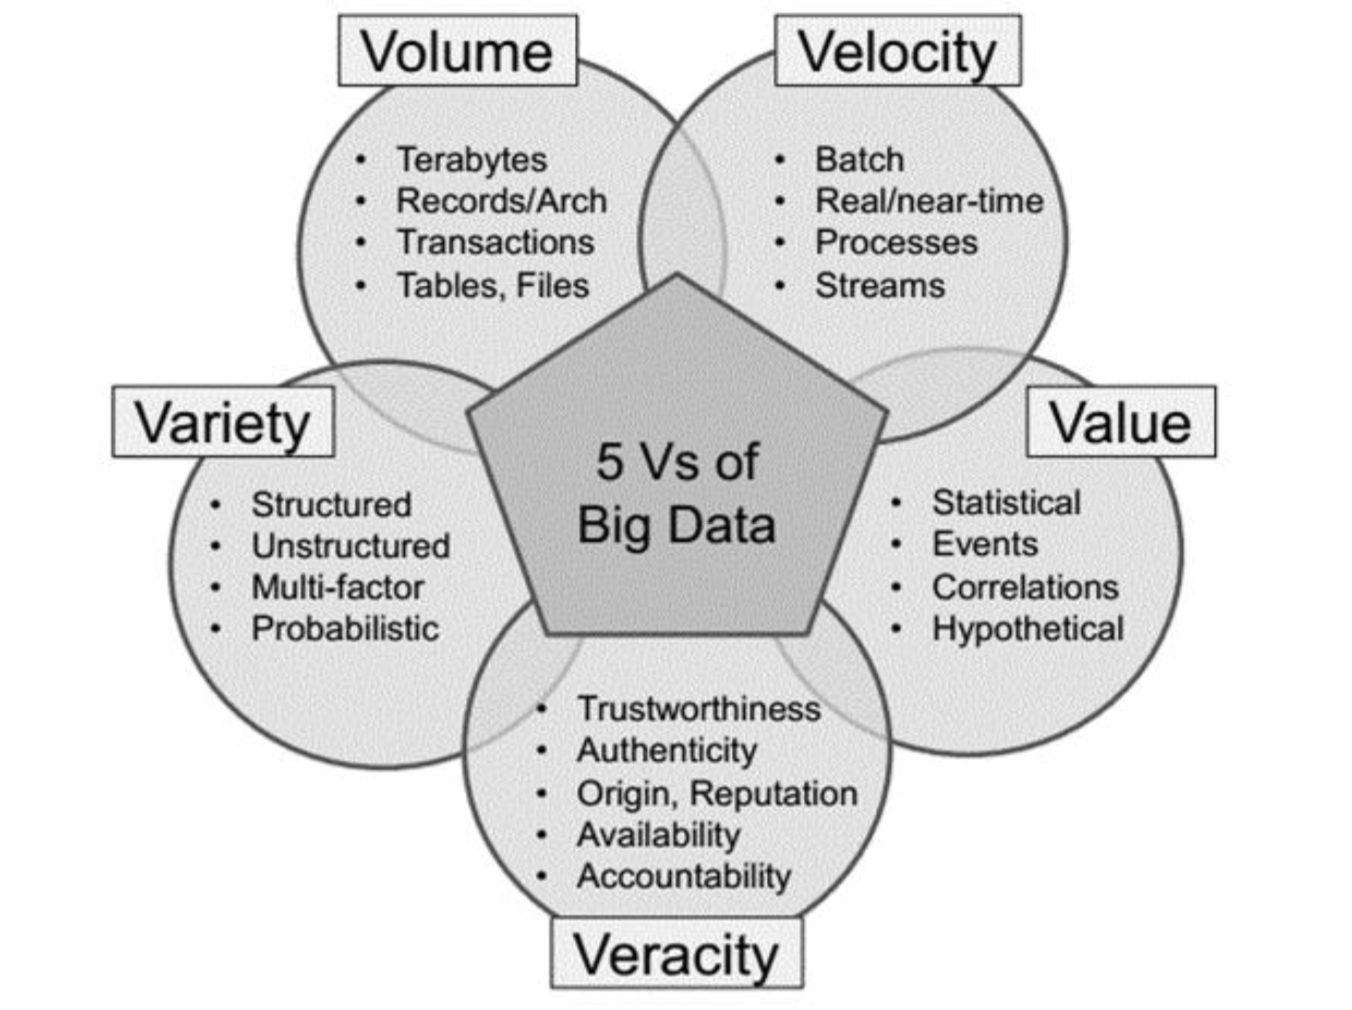
\includegraphics[width=0.75\textwidth]{{resources/big-data-parameters}.png}\par}
  \caption{The \emph{5V's} of \acl{BDA}. Reprinted from \autocite[][p.~81]{rajasekar2015survey}}
  \label{fig-5vs}
\end{figure}

As soon as data increases complexity in at least some of these dimensions, 
it qualifies for special treatment through \ac{BDA} systems. 
Although this is a common use case, as outlined in the next section, 
only few software solutions are available in the open market 
to combat these challenges. \autocite[][p.~1182 \psqq]{chen2012business},\autocite[][p.~80]{rajasekar2015survey}

\subsection{Challenges}
\label{sota-bda-challenges}

Although \ac{BDA} promises to serve as a major accelerator to companies' businesses as discussed beforehand, it is not trivial to implement and has some inherent difficulties. Based upon the challenges categorized and summarized by \autocite[p.~406\psq]{katal2013bd}, commonly recognized challenges for \ac{BDA} projects are given as follows:

\paragraph{Privacy and Security}
Labelled by Katal et al. as the most important issue to be concerned with, privacy and security aspects may have an impact not only on the feasibility of a given analytics project, but also entail serious legal consequences. Depending on the customer base and the specific environment such as country or age group, major violations of these aspects might have a significant negative impact on the company's brand sympathy and trustworthiness. The major problem identified is the possibility of analytics to generate insights about individuals they are not aware of or they do not want others to know. Basing business decisions, such as advertisement targeting or price adjustments on such insights draws attention to ethical questions -- although technical implementation of a project might be feasible, a in-depth investigation of such concerns will be needed before rolling it out. The specific privacy and security concerns, alongside relevant laws and regulations for this project work will be discussed in \vref{sec:fund:legal}.

\paragraph{Data Access and Sharing of Information}
The ability to analyze data is dependent on the presence of underlying data and requires data acquisition processes. This data acquisition might be associated with substantial costs, e.g. when paying for external access. Especially insights that are highly desired by businesses, such as benchmarks with their competitors, can usually not be performed as there is no opportunity to acquire their data. Another obstacle in the data acquisition process is to gain the general consent to be allowed to analyze a data set; the sharing of information by data providers subsequently usable to harvest them becomes desirable. However, such data sets might not necessarily be very recent or even accurate. The insight that data access and quality play a key part for the competitive advantage in a modern business world follows trivially.

\paragraph{Storage and Processing Issues}
Due to the high volume and variety of data involved in modern \ac{BDA} projects, there may be issues with both storage respectively processing it. Although the cloud offers seemingly unlimited storage for end users, it is important to view both of these aspects in conjunction, leading to the conclusion that the highly distributed storage in various data centers, locations etc. usually leads to new problems associated with the processing of the data. The desire for a system offering solutions for both of these aspects, leading to a successful and powerful analytics platform appears to be large.

\paragraph{Analytical Challenges}
The major analytical challenges companies are confronted with when dealing with Big Data are associated with the aspects of volume and variety as well. It has to be somehow decided which data should be stored and analyzed, but especially how it should be set into perspective. With large data volumes and the desire to generate new hypotheses, it is usually not clear beforehand which data points have to be regarded and might create the largest value for the organization. Furthermore, the variety of data usually requires large and expensive harmonization efforts to make data comparable or to be able to analyze it in an automated way. 

\paragraph{Skill Requirements}
Another important aspect of the implementation and feasibility of Big Data projects is the ability to execute well, thus creating actual value and acquiring reliable insights. This requires a well-trained workforce with sophisticated skills and expertise not only in the technical process of development and application, but possibly even more so in the part of harvesting results, requiring interpretative, analytical and research capabilities. Finally, even creative skills are desired, considering e.g. data visualization or exploration efforts. This skill gap poses as initial motivation for this project work; the final artifact of a program structure will focus on incorporating all these desirable aspects.

\paragraph{Technical Challenges}
According to the authors, there exist the following four major categories of technical challenges that need to be considered when preparing and performing \ac{BDA}:

\begin{enumerate}
    \item \emph{Fault Tolerance} describes the ability of a system to be tolerant to defects or errors of its underlying components. In that sense, a analytics platform has to guarantee a high level of fault tolerance, as perfect fault tolerance is not achievable. Fault tolerance is necessary to generate reliable and predictable results in the analysis process, without corrupting either the state of the system or its final results.
    \item With enormous, ever-growing data sets to process, \emph{scalability} is another major concern. Compute clusters have to adopt to varying degrees of use in order to maintain a sufficient performance level, while as storage clusters should be able to occupy the increasing data sets dumped into it. The usual procedure to achieve scalability is to join multiple smaller computing or storage nodes into a large cluster, together with some kind of cluster management that dispatches requests. Such clusters are inherently hard to operate and especially data analysis algorithms that scale well while maintaining their descriptiveness and conciseness are hard to write.
    \item The \emph{quality of data} poses as a constraint for its derived insights. Although more data points will usually provide better insights in the case of decision making and predictive analysis, quantity does not compensate quality. As the time to process data is directly correlated to the size of the underlying data set, one should strive to analyze only the minimal data set necessary for the given problem.
    \item Finally, the \emph{heterogeneity of data} becoming more and more important with Big Data prevents the usage of traditional systems that rely on data harmonization and fixed schemas. Coming up with a way to deal with such heterogeneous data is another major obstacles of \ac{BDA}.
\end{enumerate}


\section{Hadoop}

The \emph{Apache Hadoop Project} is a collection of tools that serves as a widespread platform for \ac{BDA} use cases nowadays. Contrary to common belief, Hadoop itself aims not to replace traditional \ac{OLTP} and \ac{OLAP} systems but rather complement them by offering a common platform for \ac{BDA} use cases that rely on such a massive data scale such old systems are not capable of processing anymore. Therefore, \autoref{hadoop-components} will provide a brief overview of the foundational components among a short outline of the history of Hadoop. Moreover, an overview over the Hadoop ecosystem and its most prominent applications is given in \autoref{hadoop-ecosystem}.
Subsequently, these insights will be set into context in \autoref{hadoop-assessment}, creating a value assessment of Hadoop in the scope of \ac{BDA} and \ac{BIA}.

\subsection{Core Components}
\label{hadoop-components}

Hadoop is mainly made up of two flexible and scalable core layers: \textbf{storage} and \textbf{processing}. This subsection iterates over these layers by showing the inspiration, supporting principles and derived advantages of their application.

\subsubsection{File System} 
The storage layer is formed by the so-called \acf{HDFS}, which serves as a distributed file system that may run on clusters of arbitrary sizes and is heavily inspired by Google's \ac{BFS} paper \autocite{ghemawat2003gfs}.

The first advancement of \ac{BFS} in comparison to earlier distributed file systems is to expect failure of cluster nodes to be the norm rather than an exception: This becomes especially important when running the cluster on top of so-called \enquote{commodity hardware} \autocite[p.~1]{ghemawat2003gfs}, that means comparatively cheap consumer hardware rather than expensive enterprise server equipment. This drives down the costs of the cluster, as no premiums for high-availability features and expensive support contracts have to be paid, however to the expense of reduced availability of single nodes \autocite[p.~1]{ghemawat2003gfs}. As the file system is expecting such failure, data blocks are replicated across multiple nodes, leading to an availability guarantee approaching 100 per cent as the cluster grows \autocite[p.~2]{ghemawat2003gfs}. Secondly, rather than storing hundreds of thousands of small files as with traditional file systems, \ac{BFS} is designed to work with far fewer, yet larger files, often with sizes ranging from gigabytes to terabytes \autocite[p.~2]{ghemawat2003gfs}. Furthermore, rather than using random access, the file pointer is usually moved only linearly, resulting in an append-only mode for writing data as well as batch processing for reading data \autocite[p.~2]{ghemawat2003gfs}. Finally, the file system is custom-tailored for the applications running on top of it, rather than serving as general purpose implementation \autocite[p.~2]{ghemawat2003gfs}.

Adapting these principles \ac{HDFS} was created as a seamlessly integrated, integral part of the Hadoop system. 
To implement the storage system, 
Hadoop defines two services that form the infrastructure for \ac{HDFS} which runs on the nodes.
Data in the file system is distributed among multiple \emph{datanodes} which store blocks of files.
In the cluster there is exactly on \emph{namenode} service node which keeps track of where the blocks of each file are located and how they can be retrieved.
Utilizing the principles of \emph{sharding} and \emph{replication}
the files stored in \ac{HDFS} are split into blocks and saved on multiple \emph{datanodes}. 
There can be a \emph{secondary namenode} which  mirrors the primary and can be act as a fail-over instance.
Figure \ref{fig:hdfs_read} visualized this architecture 
and illustrates how a client reads data from \ac{HDFS} 
by first contacting the \emph{namenode} and requesting the block locations 
and subsequently contacting the \emph{datanodes} directly to read the actual data.

\begin{figure}[th]
     {\centering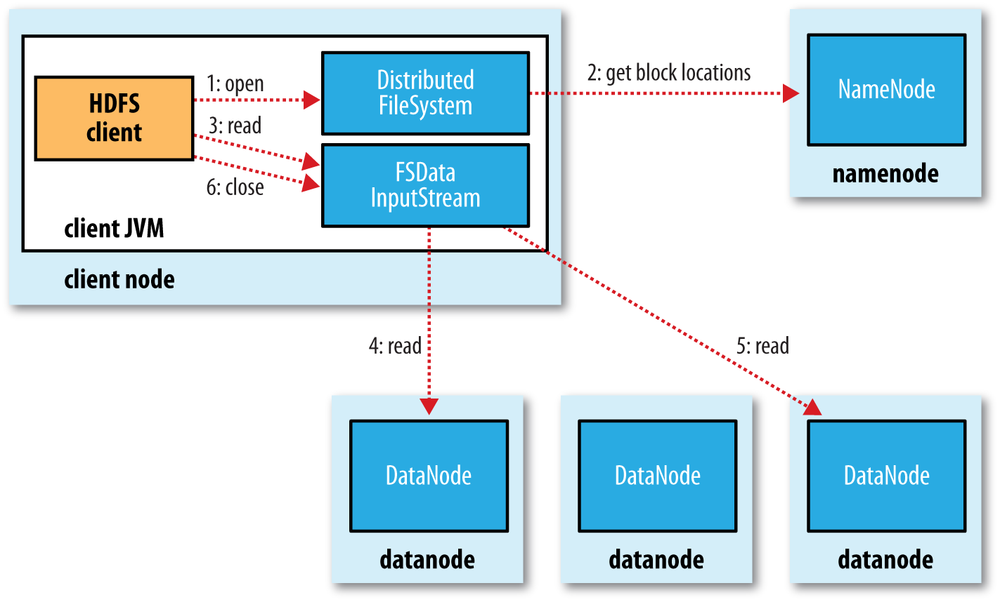
\includegraphics[width=0.75\textwidth]{img/hddg_0302.png}\par}
	\caption{\label{fig:hdfs_read}A client reading data from HDFS. Reprinted from \autocite[][Chap.~3]{white2015hadoop}}
\end{figure}

\subsubsection{Processing Framework}

Building upon this storage layer is the processing layer, which serves as the interaction point for developers, data scientists and other users of the system. The processing layer of Hadoop did undergo some major changes before the release of its second version \autocite[p.~5]{vavilapalli2013apache}; for the sake of completeness and contextual understanding both versions are subsequently outlined.

The first version of Hadoop was heavily influenced by a second important Google paper, \textcite[p.~82]{rajasekar2015survey}, introducing the batch processing algorithm MapReduce in 2004 \autocite{dean2004mapreduce}. Each MapReduce job $J: (M, R)$ with the map function $M: (k_1, v_1) \rightarrow list(k_2, v_2)$ and the reduce function $R: (k_2, list(v_2)) \rightarrow list(v_2)$ \autocite[p.~6]{dean2004mapreduce}. The job runner now calls $M$ for each data chunk in parallel on possibly many different nodes, resulting in the intermediate result. In a second step, upon completion of all map functions, the $v_2$ values are joined as a list by the value of their respective $k_2$, and subsequently passed to $R$, again running parallelized on multiple cluster nodes \autocite[p.~6]{dean2004mapreduce}. As outlined in the paper, a variety of data processing operations can be expressed very briefly and without concerning the programmer with the difficulties of writing a distributed, well-scaling algorithm \autocite[p.~6]{dean2004mapreduce}. The simplicity of the MapReduce pattern thus lead to a widespread adoption for various use cases across many industries as their primary batch processing framework, running on-top of Hadoop \autocite[p.~82]{rajasekar2015survey}.

Although the MapReduce approach is largely suitable for its intended use case of web crawling, among others, it is however not generally the best programming model to solve arbitrary data analysis and processing tasks.
As becomes obvious by the function definitions before, MapReduce jobs are limited to the analysis of isolated \enquote{data snippets}; finding or even investigating the relations and interdependence of larger data agglomeration quickly becomes a sophisticated, cumbersome task.

Due to the tight coupling of Hadoop 1's storage and processing layer, the design of Hadoop was inherently limiting its merit and the extent of applicable use cases. Thus, \ac{YARN} was developed as an abstraction layer between the traditional \ac{HDFS} storage layer and applications performing the data processing itself, creating a more flexible, powerful and even performant platform rendering the unintended use of MapReduce obsolete and limiting the scope of the MapReduce programming model to merely be one of the possible processing frameworks running on top of \ac{YARN} \autocite[p.~6]{vavilapalli2013apache}.

In 2013, \ac{YARN} was incorporated into the second major release of Hadoop \autocite{hadoopreleasenotes}, completing the transformation of Hadoop from being a limited, MapReduce-focused data processing platform to become a single, extensively applicable \ac{BDA} platform. Due to this change, creating processing frameworks as well as applications on top of Hadoop became easier to implement and maintain; furthermore, it stopped the abuse of MapReduce in earlier implementations, where massive data duplication and transient storage was required to mitigate the shortcomings of MapReduce for the holistic inspection and analysis of stored data.
Now higher level application frameworks can leverage \ac{YARN} to schedule arbitrary jobs on Hadoop and process the data stored in \ac{HDFS} with more diverse algorithms.

To implement the \ac{YARN} infrastructure, Hadoop introduces two services that can be deployed on the cluster nodes.
The \emph{ResourceManager} accepts application requests from clients and handles the management of computation resources in the cluster.
It can allocate new \emph{containers} on the cluster nodes, which encapsulate resources and execte the application .
There is only one \emph{ResourceManager} in the cluster.
Each node that performs data processing is running the \emph{NodeManager} service which receives jobs and executes them inside a \emph{container}.
If more resources are needed dynamically, the application running on the \emph{NodeManager} can request more resources from the \emph{ResourceManager}.
Figure \ref{fig:yarn} illustrates this behavior in a typical application execution.

\begin{figure}[th]
     {\centering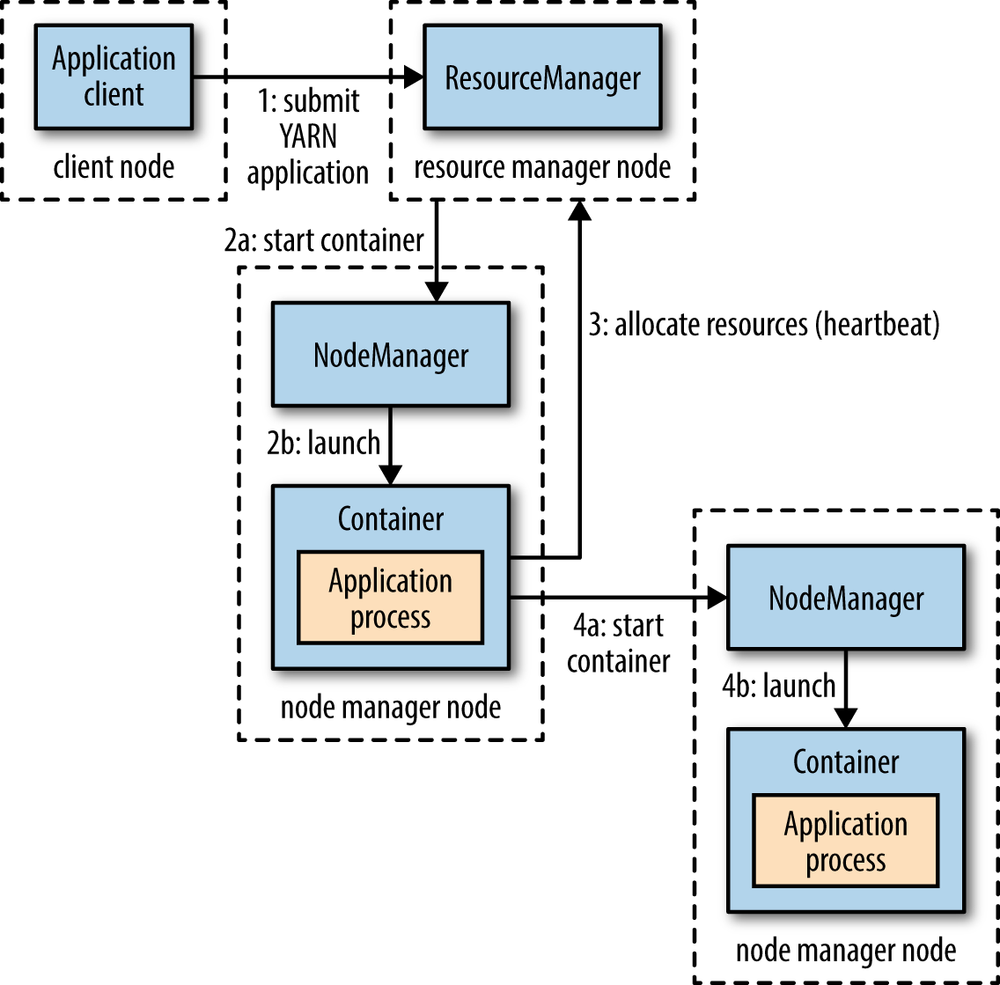
\includegraphics[width=0.75\textwidth]{img/hddg_0402.png}\par}
	\caption{\label{fig:yarn}How YARN runs an application. Reprinted from \autocite[][Chap.~4]{white2015hadoop}}
\end{figure}


\subsection{Hadoop Ecosystem}
\label{hadoop-ecosystem}

One of the major advantages of Hadoop is its rich ecosystem. 
Hadoop clusters can be extended to serve a very wide range of purposes 
that are not covered by the traditional combination of \ac{HDFS}, MapReduce and \ac{YARN}.
As Benjelloun et. al. establishes, many components in the Hadoop ecosystem 
can be grouped into the following categories.\autocite{7105553}

\paragraph{Data Integration}
Data integration tools such as \emph{Apache Flume} or \emph{Apache Sqoop} manage the transfer 
and import of large amounts of data from relational databases\autocite{apache2018sqoop}, 
event streams and other data sources\autocite{apache2017flume} into a Hadoop cluster.

\paragraph{Resource and Cluster Management}
Management tools like \emph{Apache Ambari} and \emph{Apache ZooKeeper} simplify the deployment, 
monitoring and general management of Hadoop clusters. 
Together with tools like \emph{\ac{YARN}} for low level resource management, 
and \emph{Apache Oozie} for workflow management, these tools partially define how Hadoop is used 
and are important to keep a cluster efficient.

\paragraph{Metadata Services}
This smaller category contains tools like \emph{Apache HCatalog}, 
that offer a common interface between other Hadoop data processing tools. 
Since most tools have a specific format that is used to read and write data, 
\emph{HCatalog} simplifies their integration by eliminating 
the need for manual data conversion.\autocite{bmc2017hcatalog}

\paragraph{Data Analytics}
Data analytics tools like \emph{R} work well together with Hadoop to give data scientists 
a familiar interface for analysis of the data aggregated in Hadoop. 
Additionally, machine learning frameworks like \emph{Apache Mahout} can use Hadoop 
to perform computationally expensive mathematical calculations 
on a cluster to gain deeper insights into the gathered data. 
For more simple operations, \emph{Apache Hive} can be used.

\paragraph{Search and Querying}
Search and indexing tools simplify and speed up the process of querying data stored on the \ac{HDFS}. Different tools are often optimized for a specific set of data structures and use cases. Commonly used in this context are \emph{Elasticsearch-Hadoop} or \emph{Sphinx} for full-text search, \emph{Facebook Unicorn} for graph search and \emph{Apache Hive} for \ac{SQL} like queries.

\paragraph{Data Visualization}
While data analytics tools can be used for detailed analysis, 
their usage is preceeded by data visualization tools such as \emph{Centrifuge}, 
that offer a high level overview over the available data. 
These tools can be used to discover insightful connections and visualize sections of the data.

\paragraph{Data Processing}
Since MapReduce is not the optimal choice for many kinds of workloads (cmp. \ref{sec:fund:mapred_shortcomings}), frameworks like \emph{Apache Pig} and \emph{Apache Spark} that offer a richer set of features can be used for more complicated data processing and transformation workloads. Instead of using general purpose tools, more specialized processing engines such as \emph{Apache GraphX} or \emph{Apache Giraph} can significantly improve the processing speed.

\paragraph{}
The section above mentions the most common and interesting categories of Big Data tools compatible with Hadoop. It is important to note that many tools do not fit perfectly into these categories and can often be used for multiple purposes.
The paper by \emph{Jonas Balsfulland} focuses on the usage of these tools.

\subsection{Map Reduce Shortcomings}
\label{sec:fund:mapred_shortcomings}

The growing number of Hadoop based frameworks and applications demonstrates, that using simple MapReduce based algorithms is not sufficient and flexible enough, given the amount and diversity of data gathered today. The most common issues faced by Hadoop, are caused by the limitations of the two stage MapReduce algorithm.\autocite[][]{6903263} 

MapReduce was originally developed to batch process data and is
therefore not the optimal solution to perform different kinds of
workloads that cannot be easily expressed in this
way.\autocite{computers3040117}
To approach this problem tools have been crated that follow different methods, while still utilizing \ac{HDFS} and \ac{YARN}.

In order to find an optimal solution for approaching different kinds of problems, various processing tasks usually found to be processed on Hadoop clusters may be grouped in the following ways \autocite{computers3040117}:

\paragraph{Real-time Processing}
Real-time Processing aims to reduce the response time of MapReduce jobs to allow them to be used for real-time queries and analysis. As \autocite{computers3040117} stated, one of the reasons for slow MapReduce response times is the \ac{HDFS}, which is \enquote{designed for high throughput data I/O rather than high performance I/O}.
Therefore, while MapReduce may be a powerful tool to perform batch processing, its overhead is too high to be used in any kind of real-time setting.\autocite{computers3040117}

\paragraph{Stream Processing}
While real-time processing is something MapReduce can, albeit poorly, still do, its set of features does not allow for native stream processing. MapReduce is build to run on batches of data with a very fixed cycle of:
\begin{enumerate}
    \item Gathering all the input data
    \item Running MapReduce to compute the output
    \item Returning all the output data
\end{enumerate}
This limits Hadoop with Map Reduce to use cases where all the data is known before.
However Tools such as \emph{Apache Kafka} and \emph{Apache Samza} can run on Hadoop to enable stream processing use cases with.

\paragraph{Graph Processing}
Graph processing is becoming increasingly relevant for
applications in industry and academia. 
As a general purpose computation framework Hadoop 
can be used together with MapReduce to run calculations 
on large graph datasets, 
but it generally is not optimized for such workloads.\autocite[][]{Capota:2015:GBD:2764947.2764954} 
Tools optimized for graph-like data structures can utilize algorithms that are especially optimized for graphs, instead of the general purpose MapReduce.
Examples for such tools are \emph{Apache GraphX} and \emph{Apache Giraph}.

\subsection{Value Assessment}
\label{hadoop-assessment}
The general problems and challenges with \ac{BDA} systems seen in section  \vref{sota-bda-challenges}
can also be evaluated in the context of the Hadoop platform.

\paragraph{Privacy and Security}
Hadoop has been designed as an append-only storage environment. 
This entails some serious consequences in the context of privacy, as the business desire is that individual data items should not be deleted at any time to allow for further analysis and transparency. 
In the light of recent regulations, especially relating to the \ac{GDPR} in the \ac{EU}, this is not legally compliant. 
Because of its major importance, this topic will be covered in-depth in \vref{sec:fund:legal}. The ethical questions concerned with whether to implement a certain project or not are not limited to its analytics platform and project specific and will therefore need individual judgment. 
Looking at security, it can be said that Hadoop currently does not enforce a high level of security per se, 
as neither storage nor transport level encryption are supported so far on a software level \autocite[p.~82]{rajasekar2015survey}, due to complexity and performance issues. 
However, it is possible to implement storage level encryption on a hardware level. The lack of transport level encryption however has to be noted and leads to the consequence that Hadoop clusters should be operated in a separated, 
at least virtually distinct network protected from intruders on a higher level.
On a logical level, data can be protected in \ac{HDFS} with \acp{ACL}, allowing for a granular access allocation of available data to its users \autocite{hdfspermissions}.


\paragraph{Data Access and Sharing of Information}
The ability of an organization to source external data is obviously out of scope of the analytics platform in use. However, it becomes important that Hadoop may store any data in arbitrary form, making the integration of new data sets as easy as uploading files. On an internal level, Hadoop promotes the sharing of information by offering a central data storage that should be available to any employee concerned with business development, data analytics and even more areas. Through regulatory requirements, unlimited access will be rare, however users should be made aware of the data available in order to request access if needed and legally compliant. The \emph{DataOps Manifesto} emphasizes the need of organizations to focus on viewing analytics as a processual, value-adding functional area that should always be reproducible in order to share not only the resulting knowledge but also the means of how to achieve it \autocite[][§11, §14, §17]{dataopsmanifesto}. Hadoop fits nicely into this concept, as it promotes the reuse of data and eliminates organizational boundaries that would otherwise serve as a source of operational friction.

\paragraph{Storage and Processing Issues}
This challenge area has arguably been the focus in the design and architecture of Hadoop. Therefore, Hadoop solves the capacity limits of traditional environments by offering capabilities to linearly scale the cluster's size by simply adding new nodes of commodity hardware. This positively impacts both the storage as well as the processing power. Through its sophisticated processing frameworks, including applications running on top of Hadoop for specialized use cases, a very extensive ecosystem exists to solve a wide varying array of business cases. A caveat worth noting is the maturity of this ecosystem; although some frameworks are widely used in the enterprise world and are undergoing active development, they do not have professional organization backing e.g. \acp{SLA} or other contracts that guarantee the implementation of new functionality as well as bug and security patches.

\paragraph{Analytical Challenges}
The analytical challenges can be mitigated by Hadoop only in a limited manner, as it mainly is a problem area to be addressed by business decisions (e.g. which data to upload or process). However, by offering data visualization and exploration capabilities through applications in its ecosystem as outlined in \vref{hadoop-ecosystem}, this task can be supported by Hadoop to some extent as well.

\paragraph{Skill Requirements}
Hadoop offers extensive documentation guiding users through the use of a cluster. Yet, the operation and setup of Hadoop clusters is a complex task. Later in this paper, an automated approach to this problem will be created, which can lead to a reduction of the required skill to perform the installation.
Furthermore, a substantive set of professional services firms exist on the market that may support an organization to execute the setup and maintenance of projects \autocite{hadoopconsulting}. 

\paragraph{Technical Challenges}
The four categories of technical challenges are wrapped up in \autoref{fig-hadoop-technical-challenges}. It should be noted that Hadoop addresses most of the technical challenges in a fair way, especially offering great scalability and fault tolerance. The more \enquote{soft} characteristics of quality and heterogeneity mainly rely on the best effort of the organization as well as its employees to collect the right data and use the appropriate tools offered by the Hadoop ecosystem to solve their problems.

\begin{table}[htb]
    \centering
    \resizebox{\textwidth}{!}{%
	\begin{tabular}{p{3cm}|p{7cm} p{7cm}}
	  \textbf{Characteristic} & \textbf{Advantages} & \textbf{Disadvantages} \\[0.5em]
	  \hline
	  Scalability & Supports thousands of nodes for data storage and processing. Scales almost linearly with the cluster size. High block size enables the efficient, distributed storage of vast amounts of data & Only suitable for \enquote{real} Big Data applications, not for general purpose data storage (e.g. small files)  \\
	  Fault Tolerance & Resilient to the failure of nodes, both in software and hardware (excluding the name node) & The name node serves as a single point of failure, however a secondary name node can be configured to mitigate the data loss\\
	  Quality of Data & The original data is persistently stored, and through its append-only approach, Hadoop clusters may reconstruct the data available at any point in time in order to retrospectively perform analyses & High effort for the analytics engineers to harmonize the unstructured data on-read. Mitigated in part by frameworks supporting these efforts. However, the accuracy and precision of stored data cannot be guaranteed and relies on the using organizations' policies and e.g. process steps before data is uploaded to the cluster \\
	  Heterogeneity of data & Large ecosystem of applications based on \ac{HDFS} and \ac{YARN}, covering nearly all common use cases & Parts of the ecosystem are non-mature and still under development
	\end{tabular}}
	\caption{Technical Advantages and Disadvantages of the Apache Hadoop Platform. Partly adapted from \autocite[p.~82]{rajasekar2015survey}}
	\label{fig-hadoop-technical-challenges}
\end{table}

\paragraph{Conclusion}
The points above discussed in-depth both the advantages and disadvantages of Hadoop in order to assess the aptitude of Hadoop as an analytics platform in the context of \ac{BDA}. In general, it can be said that Hadoop currently offers the most extensive and powerful solution for organizations that seek to satisfy their desire for an integrated, powerful, scalable and fault-tolerant analytics platform. The biggest problems with Hadoop itself exist in the area of \textbf{Privacy and Security}, where the current approach of an append-only environment clashes with individuals' interests for privacy, anonymity and non-interference with their personal life. Although being very mature in a technical sense, these governance and compliance problems will be of major interest in the future when organizations decide whether and how to realize their analytics efforts.

\subsection{Hadoop at the DHBW Stuttgart}

TODO welche beziehung hat die DH aktuell zu Hadoop, gibt es bereits verwendung? themen überschneidung in Vorlesungen?


\autocite[][]{DHBW2017aidbii}
DB-Implementierungen and Data Warehouse


\autocite[][]{DHBW2017aiwf}
Cloud-Anwendungen, DevOps und Bigdata

\autocite[][]{DHBW2018mannheimdatascience}
neuer studiengang auch in Stuttgart mit reaccreditierung geplang, in anlehneung zu mannheim "data science" wird sicherlich in aktuelle themen eintauchen und kann von hadoop profiteiren und behandeln


\section{Legal Boundaries}
\label{sec:fund:legal}

When a \ac{BDA} system is actively used, it handles data in diverse forms from many sources.
Depending on the kind of data, there are different legal restriction 
to the conditions of collection, storage and processing thereof.
The main restrictive laws that are applicable for the \ac{DHBW} are the Euroean \ac{GDPR}, the German \ac{BDSG} and the \ac{HSchulDSV} Baden-Würtemberg.

The \emph{\ac{HSchulDSV} in Baden-Würtemberg}  regulates which personal data the \ac{DHBW} may collect from students and how this data may be used.
It permits the usage of personal data for \enquote{organizational or other purposes} and allows the creation of anonymized reports with it.
Personal information about students must be deleted 40 years the the student was exmatriculated. 
\autocite[][§1, §11, §12]{bw2012hcchuldsv}

The \emph{German \ac{BDSG}} regulates the general principles in data protection in Germany 
and restricts the collection, usage and storage of personal data.
In general no more data than necessary may be collected and the usage requires consent. 
The user can demand the deletion of their data.
\autocite[][§1ff., §12ff.]{bmjv2009bdsg}

The \emph{European \ac{GDPR}} is largely based
on the German regulation and introduces more control for users about their personal data.
\autocite{eu2016gdpr}
The \ac{GDPR} Portal \autocite{trunomi2018gdpr} summarizes the key changes that were introduced:
\begin{itemize}
    \item \emph{Penalties} may be imposed for organizations that breach the \ac{GDPR}.
    \item \emph{Consent} from users must be requested to collection, storage and usage of personal data. The consent may be revoked.
    \item \emph{Breach Notifications} are mandatory to inform users if data was exposed.
    \item \emph{Right to Access} for every user to their own personal data.
    \item \emph{Data Portability}, i.e. the requested data should be available to the user in a common format.
    \item \emph{Right to be Forgotten}, i.e. the right to have personal data deleted permanently upon request.
    \item \emph{Privacy by Design} for new data processing systems.
\end{itemize}

Especially the \emph{right to be forgotten} is problematic in \ac{BDA} systems
since data can be stored in an unstructured, immutable way. 
This restricts the possibility to keep track of which data entries are actually stored in the system. Deletion is therefore practically impossibly. 
To circumvent this restriction, extra caution is necessary to decide which data should be used on the platform. 

The listed laws focus on personal data, but might also be applicable to anonymized data that is derived from personal data.
Table \ref{fig-legal-data-kinds} describes which restrictions regulations apply to which type of data from which source. 
An example for the kind of data is given.
Note that open source personal data sets are fundamentally not available 
since public, unrestricted distribution of personal data contradicts with the \ac{GDPR}
and no public initiative to collect such data is known to the author.

\begin{table}[hbt]
\resizebox{\textwidth}{!}{%
	\begin{tabular}{l|lll}
	  & \textbf{Internal} & \textbf{Open Source} &  \textbf{Closed Source} \\[0.5em]
	  \hline
	  \textbf{Personal} & \acs{GDPR} \& \acs{HSchulDSV} & N/A & \acs{GDPR} \& license \\
	  & e.g. student data & N/A & e.g. advertising contacts\\[0.5em]
	  \textbf{Anonymized} & possibly \acs{GDPR} \& \acs{HSchulDSV} & possibly \acs{GDPR} & possibly \acs{GDPR} \& license\\
	  & e.g. lecture statistics & e.g. social media graphs & e.g. advertising statistics\\[0.5em]
	  \textbf{Non-Personal} & unrestricted & unrestricted & restricted by license \\
	  & e.g. server monitoring & e.g. weather data & e.g. bought datasets \\
	\end{tabular}%
	}
	\caption{Kinds of data and how their use might be restricted by legislation or licenses.}
	\label{fig-legal-data-kinds}
\end{table}


When the Hadoop cluster is used at the \ac{DHBW} it might by accessed by administrative staff, lecturers and students.
However as Hadoop had not been designed with advanced user access 
and the ability to delete single records in mind,  
care must be taken to which data is stored on the Hadoop cluster.
The least restrictive solution is to use a public, open source, non-personal dataset, such as academic research data, and to avoid the storage of personal student data on the cluster. 
